\section{Characterization} \label{sec:characterization}

In this section, the Omicron algorithm is characterized. To achive this, we consider Gaussian noise and, on top of it, we inject sinusoidal Gaussian burst signals with known characteristics. This is done using the injection feature of Omicron described in Sec.~\ref{sec:algorithm:injections}. The burst waveform is given in Eq.~\ref{eq:sginj}.

\subsection{White noise} \label{sec:characterization:white}

As a first characterization, we simulate burst signals with $\phi_b$ taking random values between 32~Hz and 256~Hz, $Q_b$ between 4 and 64. The time of the injection is randomly drawn in $\pm10$~s around the chunk center. Signals are injected over a white noise data stream using a wide range of amplitude values. Then we run Omicron with the parameters listed in Appx~\ref{appx:parameters}. In the left-hand side of Fig.~\ref{}, the measured SNR is plotted against the true SNR. The plot in right-hand side of Fig.~\ref{} shows the relative SNR difference. This result is well compatible with what we obtained from Monte Carlo studies presented in Fig.~\ref{fig:snrestimator} and Tab.~\ref{tab:snrestimator}.

The signal amplitude is now fixed such that the true SNR (see Eq.\ref{eq:snr_white}) is 10 and we use fixed values for $Q_b$. 

\subsection{Colored noise} \label{sec:characterization:colored}

the amplitude spectral density of which is represented in Fig.~\ref{fig:noise_asd}. On top of this, sinusoidal Gaussian burst signals are injected. The signal expression is given by 
\begin{figure}
  \center
  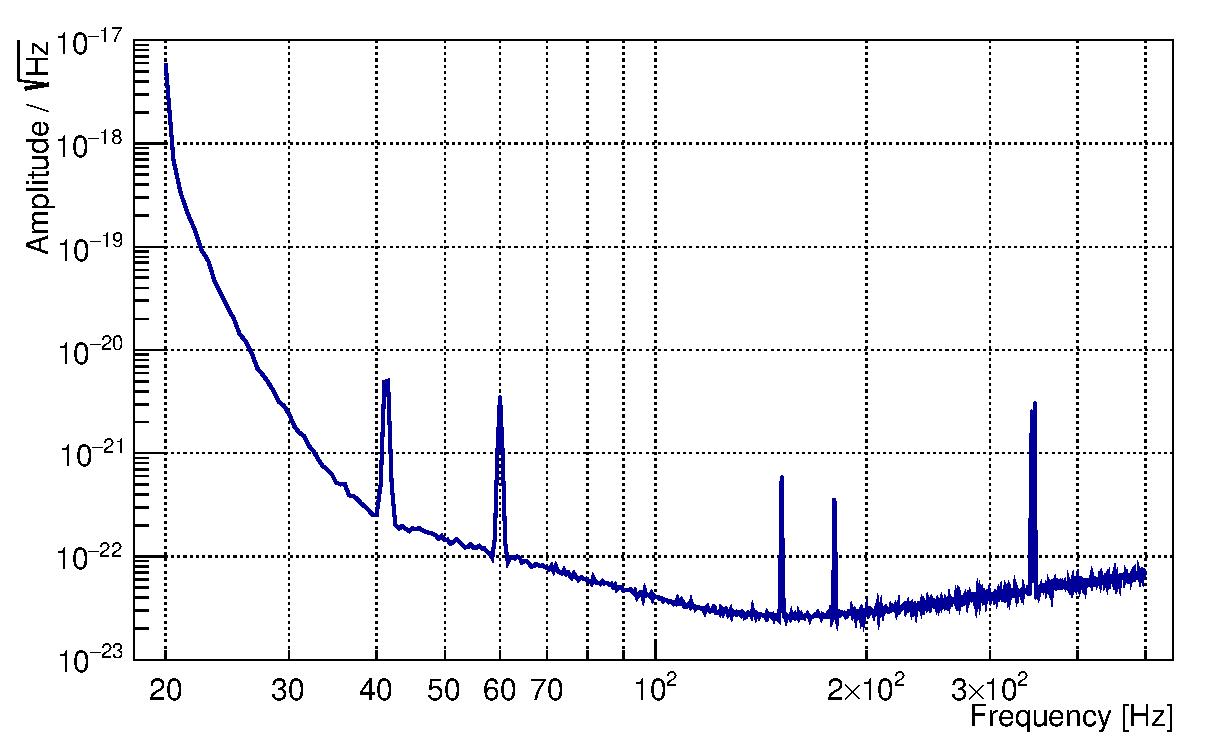
\epsfig{width=10cm, file=./figures/noise_asd.eps}
  \caption{Noise spectral density}
  \label{fig:noise_asd}
\end{figure}
